% afacs.tex
% Every number comes from files in the repository:
%   docs/data_audit.md, data/processed/audit.json        (uv run afacs-ingest)
%   docs/information_audit.md, figures/info_audit.png   (uv run afacs-info-audit)
%   results/analysis_*.md, results/agreement_*.md        (uv run afacs-analysis / afacs-agreement)
%   docs/design_check.md                                 (documentation check)
%   codebook/v1.md, codebook/v1.1.md, docs/crosswalk_ezell.md
% Compile with pdfLaTeX, twice, from the paper/ folder.
\documentclass[10pt,a4paper]{article}

\usepackage[T1]{fontenc}
\usepackage[utf8]{inputenc}
\usepackage{lmodern}
\usepackage[margin=2.5cm]{geometry}
\usepackage{amsmath,amssymb}
\usepackage{graphicx}
\usepackage{booktabs}
\usepackage{array}
\newcolumntype{L}[1]{>{\raggedright\arraybackslash}p{#1}}
\usepackage{caption}
\usepackage{float}
\usepackage{xcolor}
\usepackage{fancyhdr}
\usepackage[hidelinks]{hyperref}

\graphicspath{{../figures/}}
\captionsetup{font=small,labelfont=bf}
\setlength{\parskip}{0.35em}
\setlength{\parindent}{1.2em}

\newcommand{\code}[1]{\texttt{#1}}

\newcommand{\shorttitle}{AFACS: Incident Analysis for Multi-Agent Systems}
\pagestyle{fancy}
\fancyhf{}
\fancyhead[L]{\small\shorttitle}
\fancyhead[R]{\small J.\ Le Cuirot $\cdot$ CitadelAero}
\fancyfoot[C]{\small\thepage}
\renewcommand{\headrulewidth}{0.4pt}
\setlength{\headheight}{14pt}

\hypersetup{
  pdftitle={Extending AI-Agent Incident Analysis to Multi-Agent Systems},
  pdfauthor={James Le Cuirot (CitadelAero)}
}

\title{\vspace{-1.5em}\textbf{Extending AI-Agent Incident Analysis to Multi-Agent Systems}\\[0.3em]
\large AFACS, an HFACS-based framework, and an audit of public traces}
\author{James Le Cuirot\\
\small CitadelAero\\
\small Senior First Officer and Flight Safety Officer $\cdot$ MSc Human Factors in Aviation\\
\small \href{mailto:james@citadelaero.com}{james@citadelaero.com} $\cdot$ \href{https://citadelaero.com}{citadelaero.com}}
\date{Draft, November 2026}

\begin{document}
\maketitle
\thispagestyle{fancy}

\begin{abstract}
\noindent
Ezell, Roberts-Gaal and Chan (2025) proposed a framework for analysing incidents
involving AI agents. It treats single agents, has no category for deliberate
departures from known requirements, and has not been applied to real traces.
This paper extends it to multi-agent systems using the structure of the Human
Factors Analysis and Classification System (HFACS) from aviation. The extension,
AFACS, adds a supervision tier, a coordination category and violations coded from
behaviour with a graded statement of the evidence, and it states what evidence
each layer needs. It is tested on the public MAST dataset of multi-agent traces.
An audit finds duplicate and corrupt rows, an LLM judge that agrees with itself at
a mean Cohen's $\kappa$ of 0.43, and logs that record what the agents did but
none of the system documentation needed to reconstruct a failure. In an AI pilot,
Claude coded 250 failed traces three times. The layers were applied consistently
($\kappa$ 0.63--0.76 between two models and 0.74--0.87 between two runs of one
model; individual codes 0.52 and 0.59). Supervision failures appear in about
two-thirds of failures, coordination breakdowns in two-fifths and violations in
9--13\%, mostly inferred from the act rather than stated; MAST's ``Disobey Task
Specification'' label mixes errors with violations. Checked against the
frameworks' documentation and code, the annotator's design-level claims usually
identified a real weakness but overstated it as an absence (8 of 24 confirmed in
full, 2 contradicted): design causes need design evidence. Validation with human
coders is planned.
\end{abstract}

\section{Introduction}

When an aircraft accident is investigated, ``pilot error'' is where the analysis
starts. Reason's model of organisational accidents describes how the unsafe act
at the sharp end is made likely by latent conditions created earlier and higher
up~\cite{reason1990human,reason1997managing}. The Human Factors Analysis and
Classification System (HFACS) turned that model into a coding scheme with four
tiers, from organisational influences down to unsafe
acts~\cite{shappell2000hfacs,wiegmann2003human}. HFACS also keeps Reason's
distinction between errors, which are unintended, and violations, which are
departures from known rules. The two call for different remedies and appear to be
different kinds of behaviour~\cite{reason1990errors}.

LLM agents act over many steps: they plan, call tools, write and run code, and
exchange messages. A multi-agent system gives several agents roles, such as coder,
tester and orchestrator, much as a crew divides duties. Ezell, Roberts-Gaal and
Chan~\cite{ezell2025incident} proposed the first framework for analysing incidents
involving AI agents in this tradition. It explains incidents through system
factors, contextual factors and cognitive errors, sets out what information
investigators need, and lists open challenges. Three features leave room for
extension. It treats a single agent, so it has no place for an orchestrator that
supervises other agents or for breakdowns between agents. Its agent-level category
holds errors only: the paper cites an agent that reasoned about cheating its unit
tests before doing so~\cite{baker2025monitoring}, but no category records such a
departure. And it has not been applied to real traces.

This paper extends the framework to multi-agent systems using the structure of
HFACS, and calls the result AFACS. It takes up five of Ezell et al.'s open
challenges: non-exhaustive coverage, emerging factors, high-level cognitive
errors, reconstruction difficulties with limited data access, and, in part,
expertise shortages. Using the public MAST dataset~\cite{cemri2025mast}, it asks
four questions.
\begin{itemize}\setlength{\itemsep}{1pt}
  \item \textbf{RQ1, cross-walk.} How do Ezell et al.'s factors map onto the
  HFACS layers, and what does a multi-agent setting add?
  \item \textbf{RQ2, information adequacy.} Do real multi-agent traces contain the
  information Ezell et al.\ say investigators need?
  \item \textbf{RQ3, applicability.} Can the extended framework be applied
  consistently, and how often do failures involve the added categories?
  \item \textbf{RQ4, flat labels.} How do MAST's fourteen flat labels map onto the
  extended framework?
\end{itemize}
The contributions are the framework and its cross-walk; an audit of the MAST
dataset and of what its logs let an investigator establish; and an AI-coded pilot
on 250 traces, coded three times, with a check of the annotator's design claims
against documentation. Human validation is planned as a second study, for which a
blinded, pre-registered calibration set has been frozen.

\section{Background}

\paragraph{Incident analysis and failure taxonomies.} Ezell et al.\ define system
factors (training data, feedback, learning methods, system prompt, scaffolding),
contextual factors (information, tools, task definition) and cognitive errors
(observation, understanding, decision-making, action execution), and list
eighteen items of information investigators need (their
Table~1)~\cite{ezell2025incident}. Swiss-cheese guardrail designs and STPA look
forward, at defences and hazards~\cite{shamsujjoha2024swisscheese,leveson2012engineering,mylius2025stpa};
incident analysis looks back. MAST, derived from 150 traces, reports human
agreement of $\kappa=0.88$ and $\kappa=0.77$ between its o1 judge and
experts~\cite{cemri2025mast}, but has no causal layers. Other taxonomies classify
failures by error type~\cite{deshpande2025trail}, by the component that
broke~\cite{zhu2025agenterrorbench}, by the agent and step
responsible~\cite{zhang2025whowhen}, or by where the fix
belongs~\cite{raj2026modelharness}. They answer ``what broke'' and ``who and
when''; AFACS adds ``what kind of act'' and ``what latent conditions''.

\paragraph{HFACS and its reliability.} An aviation psychologist and a pilot
re-coding 319 causal factors from NTSB reports into HFACS agreed at
$\kappa=0.71$~\cite{wiegmann2001commercial}. Reliability is contested: a modified
HFACS showed low agreement~\cite{olsen2010hfacsadf}, and a review found it higher
with training and fewer departures from the
original~\cite{cohen2015reliability,burnham2017letter}. LLMs coding aviation
reports reach far lower exact-match than partial-match
agreement~\cite{ahmadi2025hfacsgrpo}. AFACS therefore keeps the four tiers and
reports agreement by layer as well as by code.

\paragraph{AI behaviours that resemble violations.} Specification gaming is the
standard term for many behaviours AFACS would code as
violations~\cite{krakovna2020specgaming}. ImpossibleBench builds tasks that can be
passed only by breaking the specification~\cite{zhong2025impossiblebench}.
Reasoning traces can reveal reward hacking, and models trained against monitors
learn to hide it~\cite{baker2025monitoring}. Frontier models in constructed
scenarios reason about constraints and circumvent
them~\cite{meinke2024scheming,lynch2025agentic}. OverclaimBench measures false
claims of completion with a criterion that ``requires no inference about
intent''~\cite{smyth2026overclaim}, the stance AFACS takes; and failures look
increasingly like an incoherent ``hot mess'' as tasks
lengthen~\cite{hagele2026hotmess}, so most should be errors.

\section{The AFACS Framework (RQ1)}
\label{sec:framework}

Each failed trace is coded at every layer where it gives evidence (multi-label),
with a deepest contributing layer and a confidence rating (Table~\ref{tab:codes};
\code{codebook/v1.1.md}). The codebook is the author's.

\begin{table}[tbp]
\centering
\caption{AFACS layers and codes (codebook v1, used in the pilot; v1.1 differs only in a note). L4.4, added from Ezell et al.'s
system factors, needs developer-side evidence and is not applied from traces
(Section~\ref{sec:evidence}). L4.5 covers the people who launched the run.}
\label{tab:codes}
\small
\begin{tabular}{@{}L{3.3cm}lL{9.6cm}@{}}
\toprule
Layer & Code & Description\\
\midrule
L4 Organisational / design & L4.1 & Architecture and role design: role split, missing verifier, no termination logic\\
 & L4.2 & Resource provisioning: tools, step or token budgets, context limits\\
 & L4.3 & Process: no standard procedure for verification or handover\\
 & L4.4 & Model development (developer evidence only): training data, feedback or learning methods\\
 & L4.5 & Operation set-up: the run was launched or configured wrongly, e.g.\ an empty task\\
\midrule
L3 Supervision / orchestration & L3.1 & Inadequate supervision: no check on subagent output\\
 & L3.2 & Planned inappropriate operation: task beyond an agent's capability or information\\
 & L3.3 & Failure to correct a known problem: visible loop or error, no intervention\\
 & L3.4 & Deficient specification: ambiguous, contradictory or incomplete task or prompt, set by the user or by an orchestrating agent\\
\midrule
L2 Preconditions & L2.1 & Environment: tool or API failure, bad or unavailable information\\
 & L2.2 & Agent state: context saturation, lost instructions, carried-over error\\
 & L2.3 & Coordination: communication breakdown, withheld or ignored input\\
\midrule
L1 Unsafe acts: errors & L1.E1 & Skill-based: execution slip, e.g.\ a malformed tool call\\
 & L1.E2 & Decision: wrong plan or choice given adequate information\\
 & L1.E3 & Perceptual: misread observation, tool output or message\\
L1 Unsafe acts: violations & L1.V1 & Routine: habitual shortcutting across the trace\\
 & L1.V2 & Exceptional: one-off departure, e.g.\ fabricating a result or editing tests\\
 & L1.V? & Indeterminate: the criteria appear to hold but the evidence is thin\\
\bottomrule
\end{tabular}
\end{table}

\paragraph{Adapting HFACS to multi-agent runs.}
\label{sec:people}
Five decisions adapt HFACS. (1) The humans around a run sit in existing tiers:
the user who sets the task is at the top of the supervision chain, so a deficient
task is L3.4 whoever set it, and a run launched or configured wrongly (for
instance with an empty task) is \code{L4.5} Operation set-up, the analogue of a
defective dispatch, rather than an excluded trace. (2) When the framework's own
software misbehaves, the cause decides the code: a malfunction during the run is
L2.1, a limitation in the design L4.1 or L4.2. (3) A failure need not include an
unsafe act: if a tool fails and the agents respond reasonably, no L1 code is
given. (4) A loop is the repeating agent's unsafe act and, where a supervisor
could have broken it, also L3.3. (5) An omission is coded by whose job it was: L1
if an agent was told to do it, L3.1 if a supervisor should have checked, L4.1 or
L4.3 if nobody was given the job.

\paragraph{Cross-walk.} Table~\ref{tab:crosswalk} condenses the item-by-item
mapping (\code{docs/crosswalk\_ezell.md}). Ezell et al.'s system factors map to
L4, with the system prompt treated as specification (L3.4); contextual factors to
L2.1, L3.4 and L4.2; cognitive errors to the L1 errors, with memory and
distraction at L2.2. Their four cognitive functions cut the ground differently
from HFACS's three error types, so AFACS records both for each error. In the other
direction, their model-development factor has no HFACS tier; AFACS adds L4.4 by
analogy with HFACS's resource management~\cite{wiegmann2001commercial}.

\begin{table}[tbp]
\centering
\caption{Condensed cross-walk from Ezell et al.'s factors to AFACS codes. The
last three rows have no counterpart in Ezell et al. $^{\dagger}$Needs
developer evidence; not applied from traces (Section~\ref{sec:evidence}).}
\label{tab:crosswalk}
\small
\begin{tabular}{@{}L{5.5cm}L{3.4cm}L{5.9cm}@{}}
\toprule
Ezell et al.\ factor & AFACS code & Note\\
\midrule
System: training data, feedback, learning methods & L4.4$^{\dagger}$ & Latent; feedback that rewards appearing successful is a typical condition behind violations\\
System: system prompt underspecified or encouraging undesirable behaviour & L3.4 & System prompt treated as part of the specification\\
System: scaffolding not working as intended & L4.1/L4.2 or L2.1 & Coded by cause: built into the design, or a failure during the run\\
Contextual: information inaccessible, missing, poor or malicious & L2.1 & \\
Contextual: tools unusable or failing; tool errors not visible & L2.1 or L4.2 & Run-time failure, or provisioning by design\\
Contextual: unclear or conflicting task; resource limits & L3.4; L4.2 & \\
Cognitive: observation (failure to notice, wrong expectation) & L1.E3 & Memory capacity at L2.2\\
Cognitive: understanding (misinterpretation; conclusions from poor information) & L1.E3; L1.E2 & With L2.1 where the information was poor\\
Cognitive: decision-making (goal priority, non-viable plans, criteria) & L1.E2 & Distraction from the goal at L2.2\\
Cognitive: action execution (incorrect execution; no action; no error monitoring) & L1.E1; L1.E1/E2; L1.E3 or L3.3 & L3.3 where a supervising agent should have caught it\\
\midrule
(none: single-agent framework) & L3.1--L3.3 & Orchestrator fails to check, assigns beyond capability, or leaves a visible problem uncorrected\\
(none) & L2.3 & Coordination between agents, the crew resource management analogue\\
(mentioned, not categorised) & L1.V1, L1.V2, L1.V? & Violations with an evidence grade (Section~\ref{sec:violations})\\
\bottomrule
\end{tabular}
\end{table}

\paragraph{Layered evidence.}
\label{sec:evidence}
A layered framework needs layered evidence: each layer is coded only from evidence
an investigator in that position can hold (Table~\ref{tab:evsource},
Appendix~\ref{app:tables}). Unsafe acts and preconditions are visible in the trace;
supervision failures also need the task specification and system prompt; design
factors need what is known of the design; model development needs the developer's
records. L4.4 is therefore never coded from a trace, and the annotator is never
offered it. HFACS met the same limit in aviation: organisational causes come from
company records, not the flight recorder, and were rare in NTSB-based
coding~\cite{wiegmann2001commercial}.

\paragraph{Violations.}
\label{sec:violations}
``Violation'' is used in HFACS's sense, applied to behaviour. An investigator
never sees inside a pilot's head either; a violation is inferred from evidence
that the rule was known and the action departed from it. AFACS makes no claim
about intent. A failure is a violation only if (1) the requirement was in the
agent's accessible context; (2) the trace shows the agent represented it, or the
departure cannot plausibly be accidental, such as hard-coding an expected output;
and (3) the agent proceeded otherwise. If all three hold but the evidence is thin,
the code is \code{L1.V?}; otherwise it is an error. A routine violation
(\code{L1.V1}) here means one that recurs within the run, since a single trace
cannot show a tolerated habit. The distinction matters because an error calls for
better tools, tasks or models, and a violation points to incentives, monitoring
and what training rewards. Each violation carries an evidence grade
(Table~\ref{tab:evidence}). Stated reasoning is evidence, not proof: written
reasoning may not reflect what produced an action, and models can learn to hide
it~\cite{baker2025monitoring}, which is why the \emph{inferred} grade exists.

\begin{table}[tbp]
\centering
\caption{Evidence grades for violations (codebook v1, field \code{violation\_evidence}).}
\label{tab:evidence}
\small
\begin{tabular}{@{}lL{9.8cm}l@{}}
\toprule
Grade & Use when & Goes with\\
\midrule
stated & The agent's own words (reasoning, plan or message) acknowledge the requirement, and it then departs from it & L1.V1, L1.V2\\
inferred & Nothing in the agent's words shows it registered the requirement, but the act cannot plausibly be accidental & L1.V1, L1.V2\\
thin & The criteria seem to hold but the evidence for condition (1) or (2) is weak & L1.V?\\
none & No violation is coded & \\
\bottomrule
\end{tabular}
\end{table}

\paragraph{Failures and incidents.} Ezell et al.\ analyse incidents, events that
cause or could cause harm. MAST's traces are failed benchmark tasks. Aviation
applies the same causal analysis to occurrences without harm, because their
causes are the causes of future accidents; AFACS is applied on that basis.

\section{Data and Method}
\label{sec:method}

\paragraph{Data and audit.}
\label{sec:audit}
The data are MAST's public release (\code{mcemri/MAST-Data}, revision
\code{95118ac}, CC-BY-4.0): 1{,}642 traces from seven frameworks, each with 14
binary labels from an LLM judge (o1). The audit (Appendix~\ref{app:audit};
\code{docs/data\_audit.md}) found 1{,}537 distinct traces among the 1{,}642 rows;
a group of 100 rows holding 30 distinct texts with unrelated labels; misfiled and
mislabelled traces; five runs launched with an empty task; no record of task
success; and, on 30 traces the judge labelled twice, a mean per-mode $\kappa$ of
0.43 (pooling modes would inflate it to 0.54, so per-code averaging is used
throughout). After exclusions, and excluding ChatDev (traces of 60{,}000--500{,}000
tokens) and traces over 30{,}000 tokens, the eligible pool is 893 MAST-failed
traces across six frameworks.

\paragraph{Rendering and blinding.} A parser per log format splits each trace into
numbered steps, keeping agent text verbatim. Every coder reads the same rendering.
MAST's labels are hidden, and information the agents never saw (benchmark answers
and pass/fail verdicts) is replaced by a placeholder, so that the outcome cannot
colour the coding.

\paragraph{Information audit (RQ2).} For each framework, each of Ezell et al.'s
eighteen items is classified as present, partial, absent or not applicable, using
automatic checks where reliable (timestamps, tool calls, reasoning, model
identifiers, settings, versions, errors) and otherwise three sampled traces, with
the reason recorded for every judgement (\code{docs/information\_audit.md}).

\paragraph{AI pilot (RQ3, RQ4).} Claude coded a 250-trace sample of MAST-failed
traces, balanced across frameworks and models (AG2 64, AppWorld 23, HyperAgent 13,
Magentic-One 63, MetaGPT 64, OpenManus 23), twice with \code{claude-sonnet-5-5}
and once with \code{claude-opus-5-5}, using codebook v1. Annotations ran through
Claude Code's headless mode with tools disabled and the system prompt replaced by
the annotator prompt and codebook. Replies are constrained by a JSON schema whose
allowed codes come from the codebook, and must give step-referenced quotes for
each code, a causal summary, an evidence grade for any violation, and Ezell et
al.'s cognitive function for each error. Every annotation records the models, the
prompt and codebook versions and a hash of the full instructions; a refusal is an
error, never rerouted. Each quote is checked automatically against the step it
cites. Shares are weighted back to the eligible pool and reported with Wilson
intervals (Appendix~\ref{app:method}).

\paragraph{Consistency measures.} Agreement between models and between runs uses
Cohen's $\kappa$~\cite{cohen1960kappa,landis1977measurement} for each layer's
presence, each code (averaged, never pooled), error versus violation, the evidence
grade, the deepest layer (also linearly weighted), and whether a failure was
observed, with 95\% bootstrap intervals omitted where answers are too few to
support one~\cite{feinstein1990paradox}. The share of identical full code sets is
also reported~\cite{ahmadi2025hfacsgrpo}. These measures show whether the
framework can be applied \emph{consistently}, not whether the codes are
\emph{correct}: that needs independent human coders.

\paragraph{Documentation check and worked examples.} Because the annotator sees
only the trace, its most frequent design claims for each framework were checked
against the framework's paper, documentation and code and against MAST's own
description (\code{docs/design\_check.md}). Worked examples illustrate what the
coding records, using evidence that does not depend on judging the agents' code;
they are illustrations, not validation.

\paragraph{Planned validation.} A calibration set of 30 traces (26 failed, 4 blind
MAST-clean controls; 18 development, 12 held out) was frozen before any coding,
with the hidden key's SHA-256 fingerprint committed. Independent coders will code
it blind; the AI pilot never touched it.

\section{Results}
\label{sec:results}

\subsection{RQ1: cross-walk}

Every factor in Ezell et al.'s taxonomy has a place in AFACS
(Table~\ref{tab:crosswalk}). The extension adds a supervision tier (L3.1--L3.3),
coordination between agents (L2.3) and graded violations; their framework
contributes model development (L4.4, with its own evidence requirement) and named
security contexts. In the pilot, error types and cognitive functions paired as the
cross-walk predicts (every skill-based error with action; decision errors mostly
with decision; perceptual errors with understanding and observation), but this is
not a test: the codebook the annotator read stated the prediction, and the two
schemes share examples. The prediction is removed in codebook v1.1.

\subsection{RQ2: information adequacy}

The logs are good records of what the agents said and did: responses and actions
are present in all seven frameworks (Figure~\ref{fig:info}). Everything needed to
identify or re-run the system that failed is missing. No framework provides system
documentation, artefacts or access; no framework logs a random seed; only ChatDev
logs sampling settings and system prompts; and MAST names models without versions.
The only model identifier logged inside a trace contradicts MAST's metadata for
one group of 30 traces. Labelled reasoning appears in only two frameworks, and
timestamps are absent from two (counts in Table~\ref{tab:info},
Appendix~\ref{app:tables}). For AFACS the consequence is uneven observability:
unsafe acts and coordination are well observed, supervision failures are visible
as behaviour but without prompts it is often unclear what an orchestrator was told
to do, and model development cannot be evidenced at all. These findings are an
empirical instance of Ezell et al.'s reconstruction challenge.

\begin{figure}[tbp]
\centering
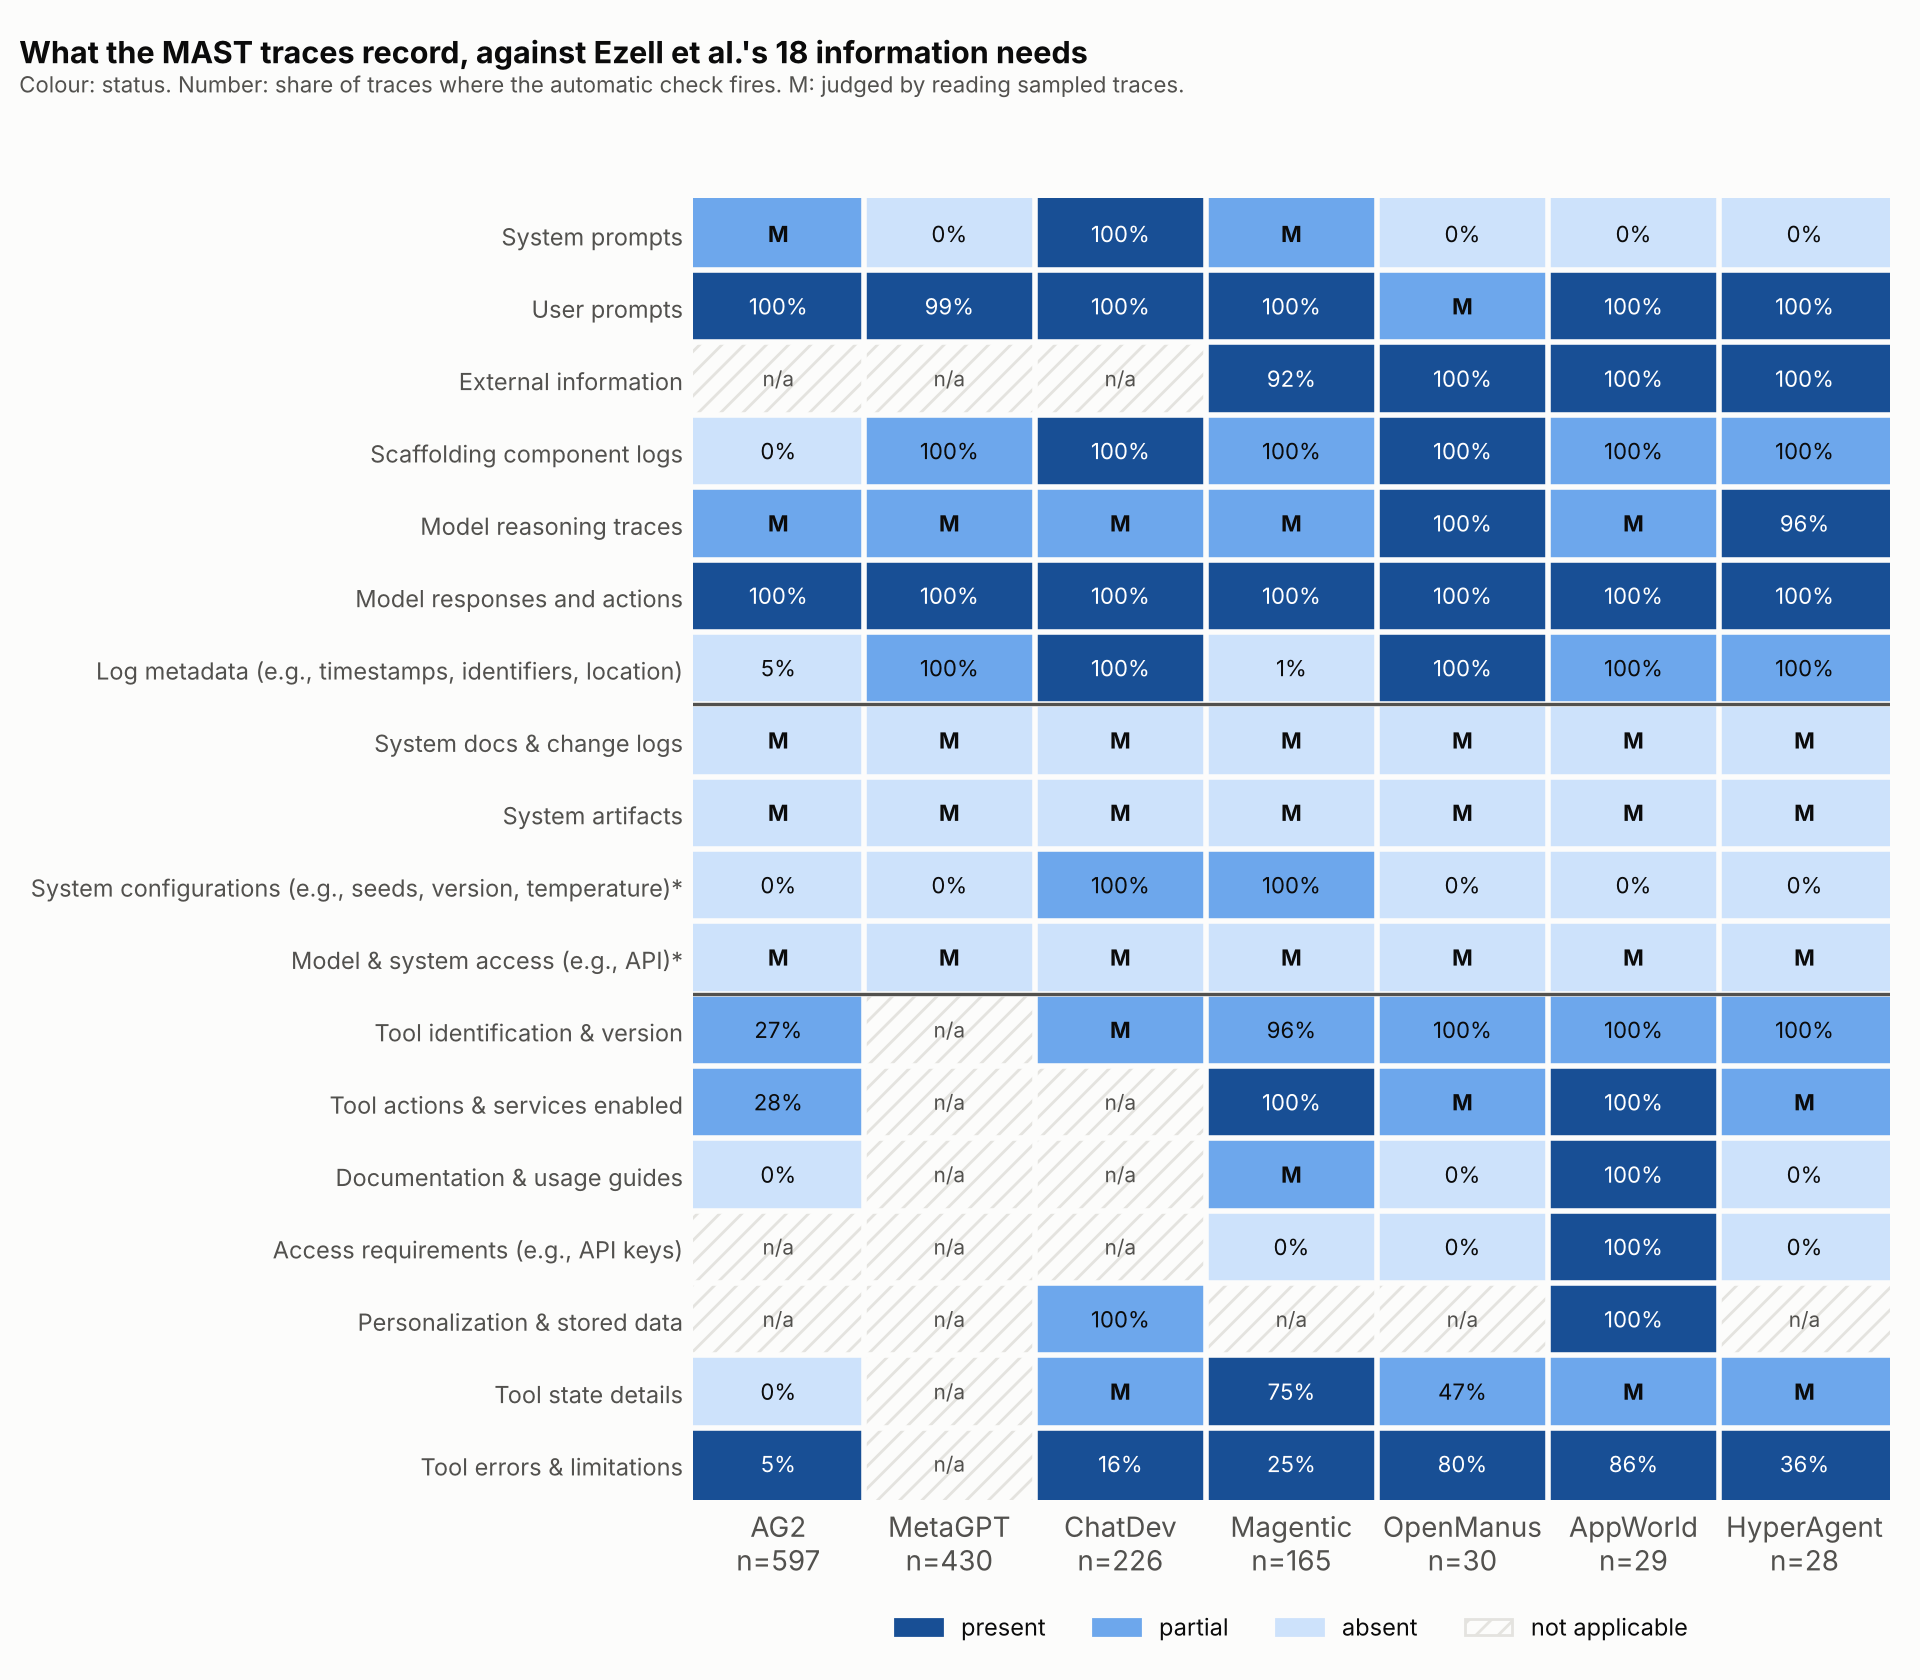
\includegraphics[width=0.72\linewidth]{info_audit.png}
\caption{MAST's logs against the eighteen information items of Ezell et al.'s
Table~1, by framework. Colour gives the status; numbers give the share of traces
in which an automatic check fires; M marks judgements made by reading sampled
traces. Items marked * matter mainly for reconstruction.}
\label{fig:info}
\end{figure}

\subsection{RQ3: applicability}

All 750 codings were valid, with no refusals or errors. Layer presence was applied
consistently (Table~\ref{tab:rq3}): $\kappa$ 0.63--0.76 between models and
0.74--0.87 between runs. Individual codes agreed less (0.52 and 0.59), the usual
pattern in HFACS coding, and 24\% and 40\% of traces received an identical full set
of codes. The weakest codes were \code{L4.3} (0.19 and 0.23), which overlaps with
\code{L4.1}; the rare \code{L1.V?} (about zero); and \code{L3.2} and \code{L3.4}
(0.32--0.62). HFACS's error types and Ezell et al.'s cognitive functions were
applied about equally consistently. The evidence was genuine: 99.6--99.9\% of about
4{,}000 quotes appeared verbatim in the step cited, and none was absent from the
trace, though the check shows that the words exist, not that they support the code.

\begin{table}[tbp]
\centering
\caption{Consistency of AI coding with AFACS on the 250-trace bulk sample.
Cohen's $\kappa$ with 95\% bootstrap intervals (2{,}000 resamples); intervals are
omitted where either coder gave fewer than three positive or negative answers.}
\label{tab:rq3}
\small
\begin{tabular}{@{}lcc@{}}
\toprule
Measure & Sonnet vs Opus & Sonnet run 1 vs run 2\\
\midrule
L4 present & 0.71 (0.62--0.79) & 0.74 (0.65--0.82)\\
L3 present & 0.63 (0.53--0.72) & 0.74 (0.65--0.82)\\
L2 present & 0.75 (0.67--0.83) & 0.76 (0.67--0.83)\\
L1 present & 0.76 (0.65--0.86) & 0.87 (0.78--0.94)\\
Individual codes (mean per-code $\kappa$) & 0.52 (0.45--0.57) & 0.59 (0.53--0.66)\\
Violation vs error & 0.67 (0.51--0.81) & 0.68 (0.50--0.83)\\
Violation evidence grade & 0.56 & 0.62\\
Error type, HFACS E1--E3 (mean per-code $\kappa$) & 0.55 & 0.71\\
Error type, Ezell et al.\ functions (mean per-label $\kappa$) & 0.58 & 0.70\\
Deepest layer (weighted) & 0.75 (0.68--0.82) & 0.80 (0.73--0.86)\\
Failure observed & 0.69 (0.57--0.79) & 0.80 (0.70--0.88)\\
Identical full code set (share of traces) & 24\% & 40\%\\
Evidence quotes found in the cited step & \multicolumn{2}{c}{Sonnet 99.6\%, 99.6\%; Opus 99.9\%}\\
\bottomrule
\end{tabular}
\end{table}

Weighted to the eligible pool, the annotator found a failure in 79--83\% of the
MAST-failed traces. Among failures, every run coded an unsafe act in all of them
and a factor at L2--L4 in 85--91\%. The categories AFACS adds were common:
supervision failures (L3.1--L3.3) in 67\% (95\% interval 59--75\%; other runs 69\%
and 71\%) and coordination breakdowns (L2.3) in 40\% (32--48\%; 41\%, 41\%).
Violations were a minority: 9\% of failures (5--15\%; 13\%, 10\%), mostly inferred
from the act (6\%) rather than stated (1\%), concentrated in HyperAgent (69\% of its
failures) and AG2 (24\%) and absent from MetaGPT and AppWorld. The typical
violation was an agent reporting results of tool calls it never received, or
``verification'' code that only returned a hard-coded answer.

Three features need care. Design factors (L4) were coded in 63--74\% of failures
and were usually the deepest layer, but every L4 code is an inference from the
trace (Section~\ref{sec:designcheck}). No run ever left L1 empty, although the
codebook allows it; the prompt's instruction to look for ``the unsafe acts at the
sharp end'' may encourage this. And confidence was ``medium'' in 86--87\% of
codings, but informative when used: for codings rated ``low'', the two Sonnet runs
agreed on whether there was a failure in 67\% of cases, against 96\% for
``medium''.

\subsection{Design claims against documentation}
\label{sec:designcheck}

Only two of the annotator's 24 most frequent design claims were wrong outright,
but only eight held in full (Table~\ref{tab:designcheck}). The typical error was
to overstate a weakness as an absence: ``no verifier'', ``no termination logic'' or
``no loop detection'' where the system has the mechanism in a weak form. MetaGPT's
reviewer comments only on the tests; MathChat detects repeated results;
Magentic-One's orchestrator asks itself each turn whether it is in a loop;
OpenManus has a duplicate-response detector that only adds a prompt; HyperAgent's
editor rejects edits that fail a syntax check. A weak mechanism that fails leaves
the same trace as a missing one. Two claims placed a failure at the wrong layer (a
run-time fault and an environment set-up problem coded as design), and the
annotator missed limits that no trace reveals, such as Magentic-One's 20-turn
budget. Design factors coded from traces should be read as ``no effective
safeguard visible in the trace''. The check also exposed discrepancies in MAST's
own documentation (Appendix~\ref{app:audit}): MetaGPT ran as a three-role example
with no verifier of the code, and the HyperAgent traces carry a model label that
postdates their source.

\begin{table}[tbp]
\centering
\caption{The annotator's most frequent design claims checked against each
framework's documentation and code.}
\label{tab:designcheck}
\small
\begin{tabular}{@{}lrrrrr@{}}
\toprule
Framework & Claims & Confirmed & Partly true & Contradicted & Not settled\\
\midrule
MetaGPT & 5 & 2 & 3 & 0 & 0\\
AG2 & 4 & 1 & 2 & 1 & 0\\
Magentic-One & 6 & 2 & 3 & 1 & 0\\
OpenManus & 4 & 2 & 2 & 0 & 0\\
HyperAgent & 3 & 0 & 3 & 0 & 0\\
AppWorld & 2 & 1 & 0 & 0 & 1\\
\midrule
All & 24 & 8 & 13 & 2 & 1\\
\bottomrule
\end{tabular}
\end{table}

\subsection{RQ4: MAST's flat labels}

Every MAST mode spread across layers (Figure~\ref{fig:crosswalk}; expectations in
Table~\ref{tab:expect}, Appendix~\ref{app:tables}). FM-1.1 Disobey Task
Specification ($n=79$) was a mixture: 17\% of its traces carry a violation code
(22\% and 12\% in the other runs) and the rest errors only, while a deficient
specification was coded in only 6\%. L2.3 coordination appears in 52\% of FM-2.3
Task Derailment and 62\% of FM-2.5 Ignored Other Agent's Input. FM-1.3 Step
Repetition was coded as a design factor (L4.1, 60\%) more often than as a
supervisor failing to break the loop (L3.3, 27\%), and FM-3.2 No or Incomplete
Verification split between supervision (L3.1, 69\%) and design (L4.1, 69\%). A
single flat label therefore covers failures whose remedies differ: a missing
verifier, a supervisor who did not check, and an agent that departed from a
requirement it had registered.

\begin{figure}[tbp]
\centering
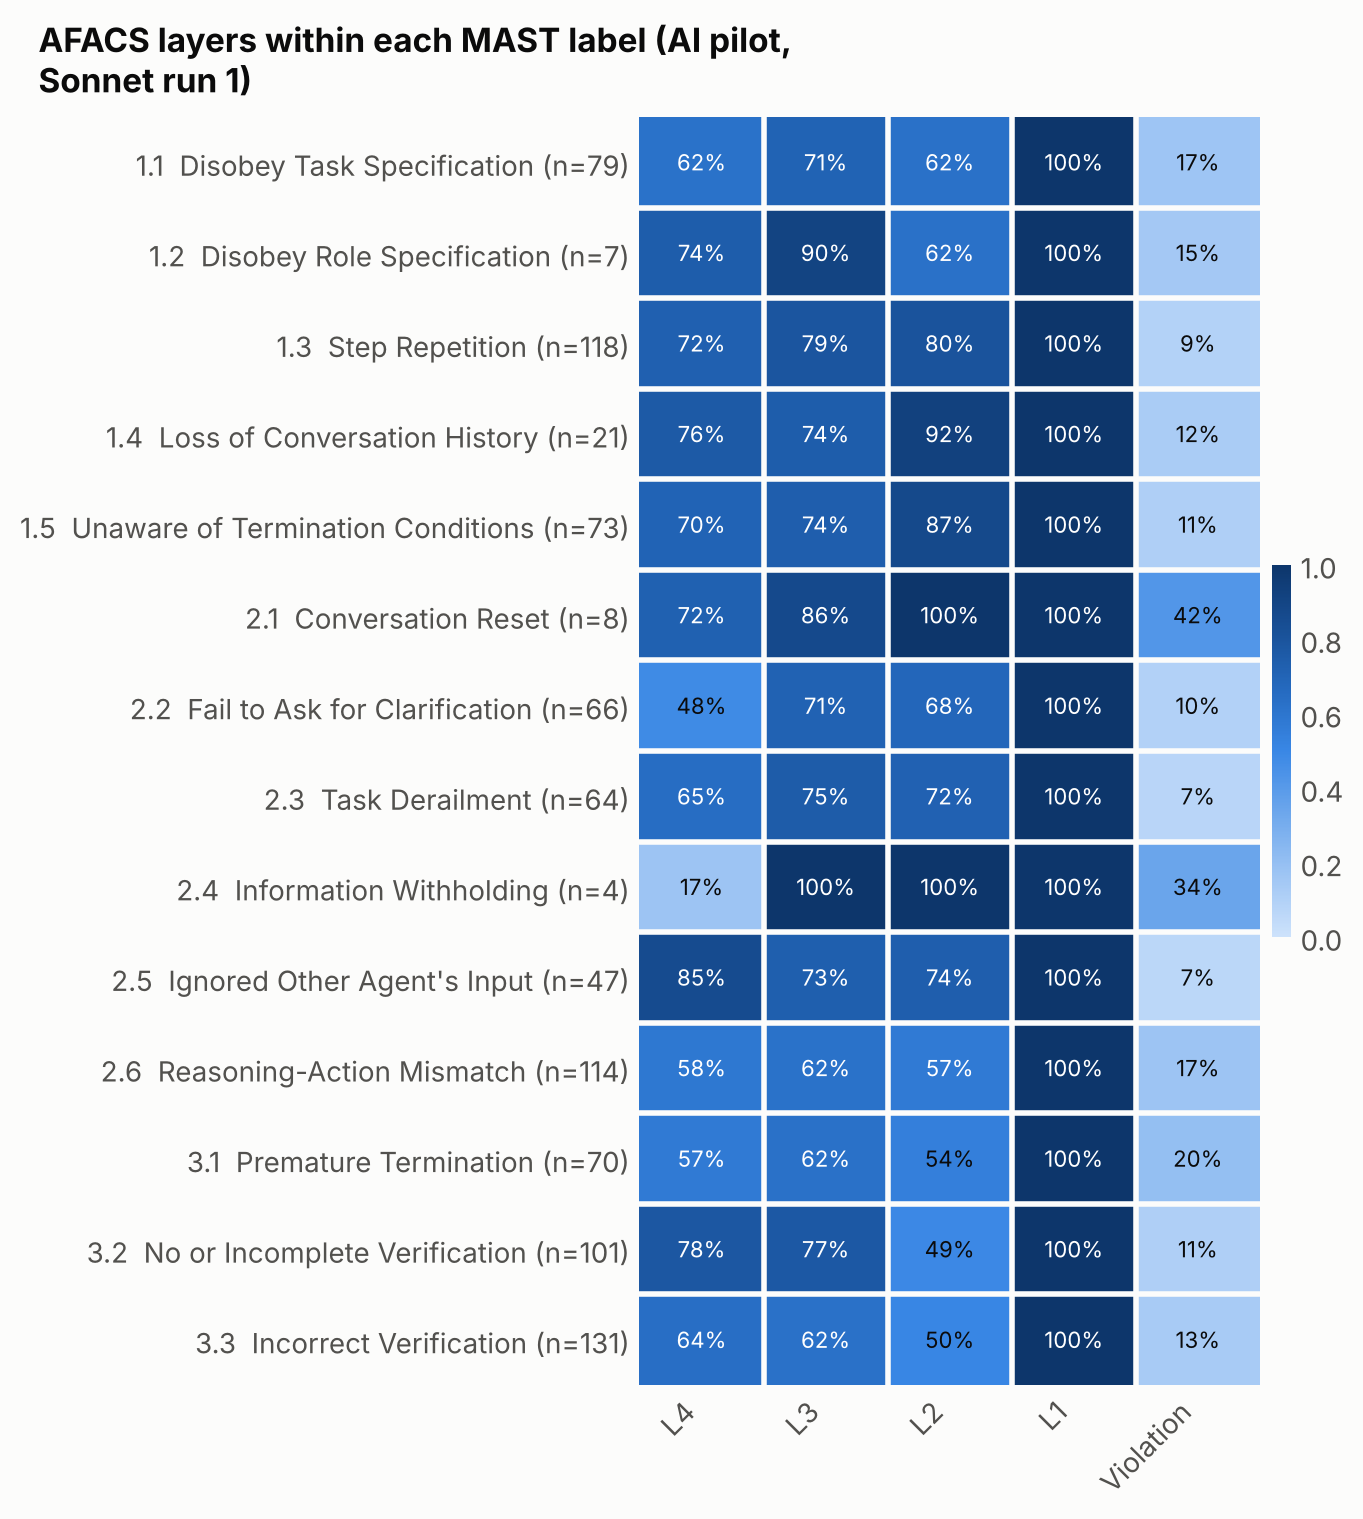
\includegraphics[width=0.62\linewidth]{crosswalk_layers_sonnet_bulk_r1.png}
\caption{Share of failed traces carrying each MAST label that have an AFACS factor
at each layer, and a violation code (Sonnet run 1, weighted).}
\label{fig:crosswalk}
\end{figure}

\section{Worked Examples}
\label{sec:cases}

Three short traces, each coded alike by all three runs, show what the layered
coding records. Each statement rests on the trace, the benchmark's verdict or the
documentation; benchmark questions are not reproduced. Two further examples are in
Appendix~\ref{app:cases}.

\paragraph{A failure built into the design (MetaGPT).} In
\code{MetaGPT\_ProgramDev-v2\_Qwen\_\_043} the task is a command-line weight
converter. The coder's table covers eight direct unit pairs and rejects any other
(S3). After the reviewer suggests testing an indirect conversion (S5), the tester
adds a test for kilograms to ounces (S6), a pair the table lacks, so the test
would fail; nobody can find out, because no agent runs code. The reviewer then
replies in another language, approves the tests and reports a syntax error that is
not there (S7), and the run ends with the code unrevised. MAST labels the trace
2.6, 3.1 and 3.3. All three runs code L4.1 (nothing runs or checks the code, and
the review never reaches the coder), L3.1 (the only check never checked the code)
and L1 errors; the documentation confirms the design claim. The flat labels name
symptoms; the layered account places the deepest cause in a design that makes them
likely whatever the agents do.

\paragraph{Flagged, but passed (AppWorld).} MAST's judge labelled
\code{AppWorld\_Test-C\_GPT-4o\_\_000} 2.6 Reasoning--action mismatch, placing it
among MAST's failed traces. The benchmark's own evaluation, hidden from the agents
and the annotator, says the task passed, and all three runs judged that no failure
occurred, noting inefficiencies but no unsafe act. Three of the 23 AppWorld traces
in the sample passed despite MAST labels, and the annotator's judgement matched the
benchmark in 21 of 23. A list of failure modes records what a judge noticed, not
whether anything failed; AFACS records the two separately, as an occurrence report
does.

\paragraph{A missing tool, or a tool not used (Magentic-One).} In
\code{Magentic\_One\_GPT4o\_\_029} the task needs information in an image file. The
orchestrator twice asks FileSurfer to read it (S5, S7); FileSurfer replies that it
cannot interpret images (S8). A text-recognition tool installed instead garbles the
part that matters (S11--S12), the assistant works from the garbled text (S14), and
the orchestrator submits an unchecked answer (S15). All three runs code a missing
tool (L4.2) as the deepest factor. The documentation qualifies this: WebSurfer
works from screenshots and can open local files, and it was never asked. On that
evidence the account should also include the orchestrator assigning the task to an
agent that could not do it (L3.2), which only one run coded. Design claims made
from a trace need the system's documentation.

\section{Discussion}

The extension earns its place. The categories with no counterpart in Ezell et
al.'s framework were among the most frequently coded, and violations, though rare,
were where MAST's labels were least informative; the evidence grade showed that
most rested on the act rather than on stated reasoning. An AI annotator applied
the layers consistently, well above MAST's judge on its own labels. Two cautions
temper this. Consistency is not correctness. And the deeper the layer, the less a
trace can establish: design factors were the most common deepest layer yet the
least observable, and the documentation check showed what trace-only coding gets
wrong. In aviation, organisational findings come from company records rather than
the flight recorder; the same division of evidence applies here. For the field,
the information audit suggests a logging standard for multi-agent research
releases, covering at least model identifiers and versions, sampling settings and
seeds, system prompts and role definitions, and timestamps.

\section{Limitations}

\begin{itemize}\setlength{\itemsep}{1pt}
  \item \textbf{Consistency, not correctness.} Agreement between AI runs can
  coexist with shared error; human validation is the next study. The annotator is
  a language model coding other language models and may share their blind spots.
  \item \textbf{Inferred design factors.} L4 codes are inferences from traces and,
  checked against documentation, tend to overstate absences.
  \item \textbf{No failure without an unsafe act was coded,} although the codebook
  allows it; whether such failures are rare or the option is avoided is open.
  \item \textbf{Outcomes were hidden} to avoid hindsight bias, so the annotator
  could not tell whether, for example, a mathematical answer was wrong.
  \item \textbf{The Ezell pairing is not a test,} because the codebook the
  annotator read stated it.
  \item \textbf{Behavioural, not intentional.} ``Violation'' describes the trace,
  not what a model wanted.
  \item \textbf{Data.} MAST's labels are noisy and record no outcome; ChatDev and
  long traces are excluded; model is confounded with framework; benchmark failures
  carry no harm; and HFACS's own reliability is debated.
  \item \textbf{Annotation route.} Annotations ran through Claude Code's headless
  mode; results through the bare API may differ slightly.
\end{itemize}

\section{Future Work}

The next study validates AFACS with independent human coders on the frozen
calibration set. Three questions from the pilot belong there: how often
trace-inferred design factors are right, when each trace is reviewed with the
system's documentation; whether failures without an unsafe act are rare or induced
by the prompt, tested with a variant prompt; and how coding changes when the
annotator knows the outcome (the verdict, not the answer), as an investigator knows
an accident occurred, or uses datasets with verified outcomes and human
attribution~\cite{zhang2025whowhen}. A fifth level for the people around a system
(users, operators, regulators) may suit deployed systems better and is left open.
A further phase will apply AFACS to an evaluation of aviation dispatch and safety
decisions under commercial, authority and user pressure, built in
Inspect~\cite{aisi2024inspect} from public regulatory sources; related aviation
evaluations~\cite{brooker2026preflight,wu2026pilotbench,yuan2026aerocopilotbench}
do not code their failures with a human-factors framework.

\section*{Competing Interests}

The author's company, CitadelAero, works on AI for aviation, the area of the
aviation evaluation proposed as future work. This study received no external
funding and uses only public data.

\section*{Use of AI Tools}

The data pipeline, tests, figures and much of the drafting were done with Claude
Code under the author's direction. The pilot's annotations were produced by Claude
models as described in Section~\ref{sec:method}. The worked examples and the
documentation check were prepared with Claude and checked against the traces and
sources they cite. The framework and the codebook decisions are the author's.

\section*{Data and Code}

Code: MIT licence, \textcopyright{} 2026 CitadelAero Limited, at
\url{https://github.com/JamesLeCuirot/Research}. Data: MAST dataset, Cemri et
al.~\cite{cemri2025mast}, CC-BY-4.0. Traces are not redistributed, because they
contain benchmark questions whose maintainers ask that they not be reposted; the
pipeline recreates them from the pinned revision. The AI codings are committed
with their codes in plain text and their quotes encoded, with a canary string.

\begin{thebibliography}{99}\small\setlength{\itemsep}{1pt}
\bibitem{reason1990human} J. Reason, \emph{Human Error}. Cambridge University Press, 1990.
\bibitem{reason1997managing} J. Reason, \emph{Managing the Risks of Organizational Accidents}. Ashgate, 1997.
\bibitem{shappell2000hfacs} S.~A. Shappell and D.~A. Wiegmann, ``The Human Factors Analysis and Classification System--HFACS,'' U.S. Department of Transportation, Federal Aviation Administration, Office of Aviation Medicine, Report DOT/FAA/AM-00/7, 2000.
\bibitem{wiegmann2003human} D.~A. Wiegmann and S.~A. Shappell, \emph{A Human Error Approach to Aviation Accident Analysis: The Human Factors Analysis and Classification System}. Ashgate, 2003.
\bibitem{reason1990errors} J. Reason, A. Manstead, S. Stradling, J. Baxter and K. Campbell, ``Errors and violations on the roads: a real distinction?'' \emph{Ergonomics}, vol.~33, no.~10--11, pp.~1315--1332, 1990.
\bibitem{ezell2025incident} C. Ezell, X. Roberts-Gaal and A. Chan, ``Incident analysis for AI agents,'' in \emph{Proc. AAAI/ACM Conference on AI, Ethics, and Society (AIES)}, 2025. arXiv:2508.14231.
\bibitem{baker2025monitoring} B. Baker, J. Huizinga, L. Gao, Z. Dou, M.~Y. Guan, A. Madry, W. Zaremba, J. Pachocki and D. Farhi, ``Monitoring reasoning models for misbehavior and the risks of promoting obfuscation,'' arXiv:2503.11926, 2025.
\bibitem{cemri2025mast} M. Cemri, M.~Z. Pan, S. Yang, L.~A. Agrawal, B. Chopra, R. Tiwari, K. Keutzer, A. Parameswaran, D. Klein, K. Ramchandran, M. Zaharia, J.~E. Gonzalez and I. Stoica, ``Why do multi-agent LLM systems fail?'' in \emph{Advances in Neural Information Processing Systems (NeurIPS)}, 2025. arXiv:2503.13657.
\bibitem{shamsujjoha2024swisscheese} M. Shamsujjoha, Q. Lu, D. Zhao and L. Zhu, ``Swiss cheese model for AI safety: A taxonomy and reference architecture for multi-layered guardrails of foundation model based agents,'' arXiv:2408.02205, 2024.
\bibitem{mylius2025stpa} S. Mylius, ``Systematic hazard analysis for frontier AI using STPA,'' arXiv:2506.01782, 2025.
\bibitem{leveson2012engineering} N.~G. Leveson, \emph{Engineering a Safer World: Systems Thinking Applied to Safety}. MIT Press, 2012.
\bibitem{deshpande2025trail} D. Deshpande, V. Gangal, H. Mehta, J. Krishnan, A. Kannappan and R. Qian, ``TRAIL: Trace reasoning and agentic issue localization,'' arXiv:2505.08638, 2025.
\bibitem{zhu2025agenterrorbench} K. Zhu et al., ``Where LLM agents fail and how they can learn from failures,'' arXiv:2509.25370, 2025.
\bibitem{zhang2025whowhen} S. Zhang et al., ``Which agent causes task failures and when? On automated failure attribution of LLM multi-agent systems,'' in \emph{Proc. ICML}, PMLR vol.~267, pp.~76583--76599, 2025.
\bibitem{raj2026modelharness} H. Raj, V. Gupta, A. Mahmoud, R.-G. Dumitru, D. Yi, A. Sabharwal and Y. He, ``Model or harness? An interaction-centric taxonomy for localizing agent failures,'' arXiv:2607.28802, 2026.
\bibitem{wiegmann2001commercial} D.~A. Wiegmann and S.~A. Shappell, ``A human error analysis of commercial aviation accidents using the Human Factors Analysis and Classification System (HFACS),'' U.S. Department of Transportation, Federal Aviation Administration, Office of Aviation Medicine, Report DOT/FAA/AM-01/3, 2001.
\bibitem{olsen2010hfacsadf} N.~S. Olsen and S.~T. Shorrock, ``Evaluation of the HFACS-ADF safety classification system: Inter-coder consensus and intra-coder consistency,'' \emph{Accident Analysis \& Prevention}, vol.~42, no.~2, pp.~437--444, 2010.
\bibitem{cohen2015reliability} T.~N. Cohen, D.~A. Wiegmann and S.~A. Shappell, ``Evaluating the reliability of the Human Factors Analysis and Classification System,'' \emph{Aerospace Medicine and Human Performance}, vol.~86, no.~8, pp.~728--735, 2015.
\bibitem{burnham2017letter} B.~R. Burnham, ``Letter to the Editor re: Evaluating the reliability of the Human Factors Analysis Classification System,'' \emph{Aerospace Medicine and Human Performance}, vol.~88, no.~6, p.~597, 2017.
\bibitem{ahmadi2025hfacsgrpo} A. Ahmadi, S. Sharif and Y. Banad, ``Improving aviation safety analysis: Automated HFACS classification using reinforcement learning with group relative policy optimization,'' arXiv:2508.21201, 2025.
\bibitem{krakovna2020specgaming} V. Krakovna, J. Uesato, V. Mikulik, M. Rahtz, T. Everitt, R. Kumar, Z. Kenton, J. Leike and S. Legg, ``Specification gaming: the flip side of AI ingenuity,'' DeepMind blog, April 2020.
\bibitem{zhong2025impossiblebench} Z. Zhong, A. Raghunathan and N. Carlini, ``ImpossibleBench: Measuring LLMs' propensity of exploiting test cases,'' arXiv:2510.20270, 2025.
\bibitem{meinke2024scheming} A. Meinke, B. Schoen, J. Scheurer, M. Balesni, R. Shah and M. Hobbhahn, ``Frontier models are capable of in-context scheming,'' arXiv:2412.04984, 2024.
\bibitem{lynch2025agentic} A. Lynch, B. Wright, C. Larson, S.~J. Ritchie, S. Mindermann, E. Hubinger, E. Perez and K. Troy, ``Agentic misalignment: How LLMs could be insider threats,'' arXiv:2510.05179, 2025.
\bibitem{smyth2026overclaim} N. Smyth et al., ``Quantifying overclaiming propensity in frontier LLM agents,'' arXiv:2609.20812, 2026.
\bibitem{hagele2026hotmess} A. Hägele, A.~P. Gema, H. Sleight, E. Perez and J. Sohl-Dickstein, ``The hot mess of AI: How does misalignment scale with model intelligence and task complexity?'' in \emph{Proc. ICLR}, 2026. arXiv:2601.23045.
\bibitem{cohen1960kappa} J. Cohen, ``A coefficient of agreement for nominal scales,'' \emph{Educational and Psychological Measurement}, vol.~20, no.~1, pp.~37--46, 1960.
\bibitem{landis1977measurement} J.~R. Landis and G.~G. Koch, ``The measurement of observer agreement for categorical data,'' \emph{Biometrics}, vol.~33, no.~1, pp.~159--174, 1977.
\bibitem{feinstein1990paradox} A.~R. Feinstein and D.~V. Cicchetti, ``High agreement but low kappa: I. The problems of two paradoxes,'' \emph{Journal of Clinical Epidemiology}, vol.~43, no.~6, pp.~543--549, 1990.
\bibitem{aisi2024inspect} UK AI Security Institute, ``Inspect AI: Framework for large language model evaluations,'' software, 2024. \url{https://inspect.aisi.org.uk/}.
\bibitem{brooker2026preflight} A. Brooker and T. Hughes, ``Pre-Flight: A benchmark for evaluating large language models on aviation operational knowledge,'' arXiv:2607.01829, 2026.
\bibitem{wu2026pilotbench} Y. Wu, H. Liu, Z. Li and B. Wang, ``PilotBench: A benchmark for general aviation agents with safety constraints,'' in \emph{Proc. International Joint Conference on Neural Networks (IJCNN)}, 2026. arXiv:2604.08987.
\bibitem{yuan2026aerocopilotbench} Y. Yuan, Z. Wu, Y. Li, L. Ma and K. Li, ``AeroCopilotBench: Safety-gated evaluation of LLM agents on aircraft emergency procedures in an executable cockpit,'' arXiv:2608.16349, 2026.
\end{thebibliography}

\appendix

\section{Data Audit Details}
\label{app:audit}

\begin{table}[tbp]
\centering
\caption{Data-quality exclusions applied before sampling.}
\label{tab:exclusions}
\small
\begin{tabular}{@{}lrl@{}}
\toprule
Reason & Rows & Note\\
\midrule
Kept & 1{,}505 & \\
Corrupt source group & 96 & ChatDev--CodeLlama: 100 rows hold 30 distinct texts\\
Duplicate text & 35 & identical trajectory seen earlier; first copy kept\\
No MAST labels & 4 & all 14 labels null\\
Misfiled text & 2 & ``HyperAgent'' rows that contain ChatDev logs\\
\midrule
Total & 1{,}642 & \\
\bottomrule
\end{tabular}
\end{table}

\paragraph{Duplicates and judge consistency.} The 1{,}642 rows contain 1{,}537
distinct texts. Among labelled rows, 65 groups of byte-identical texts cover 166
rows, and in 59 the copies carry different labels. Thirty Magentic-One traces
appear under two group names and were labelled in separate judge runs: per-mode
$\kappa$ averages 0.43 (range $-0.05$ to 0.67; raw agreement 0.80; only 4 of 30
pairs identical; Figure~\ref{fig:retest}). MAST reports $\kappa=0.77$ between its
judge and experts~\cite{cemri2025mast}; the figures cover different traces and
are not directly comparable, but repeat runs disagreeing this much suggest
substantial run-to-run noise in individual labels. In the ChatDev--CodeLlama group,
copies of the same text agree at $-0.04$ over 111 pairs, suggesting texts and
labels were mismatched upstream; the group is excluded.

\begin{figure}[tbp]
\centering
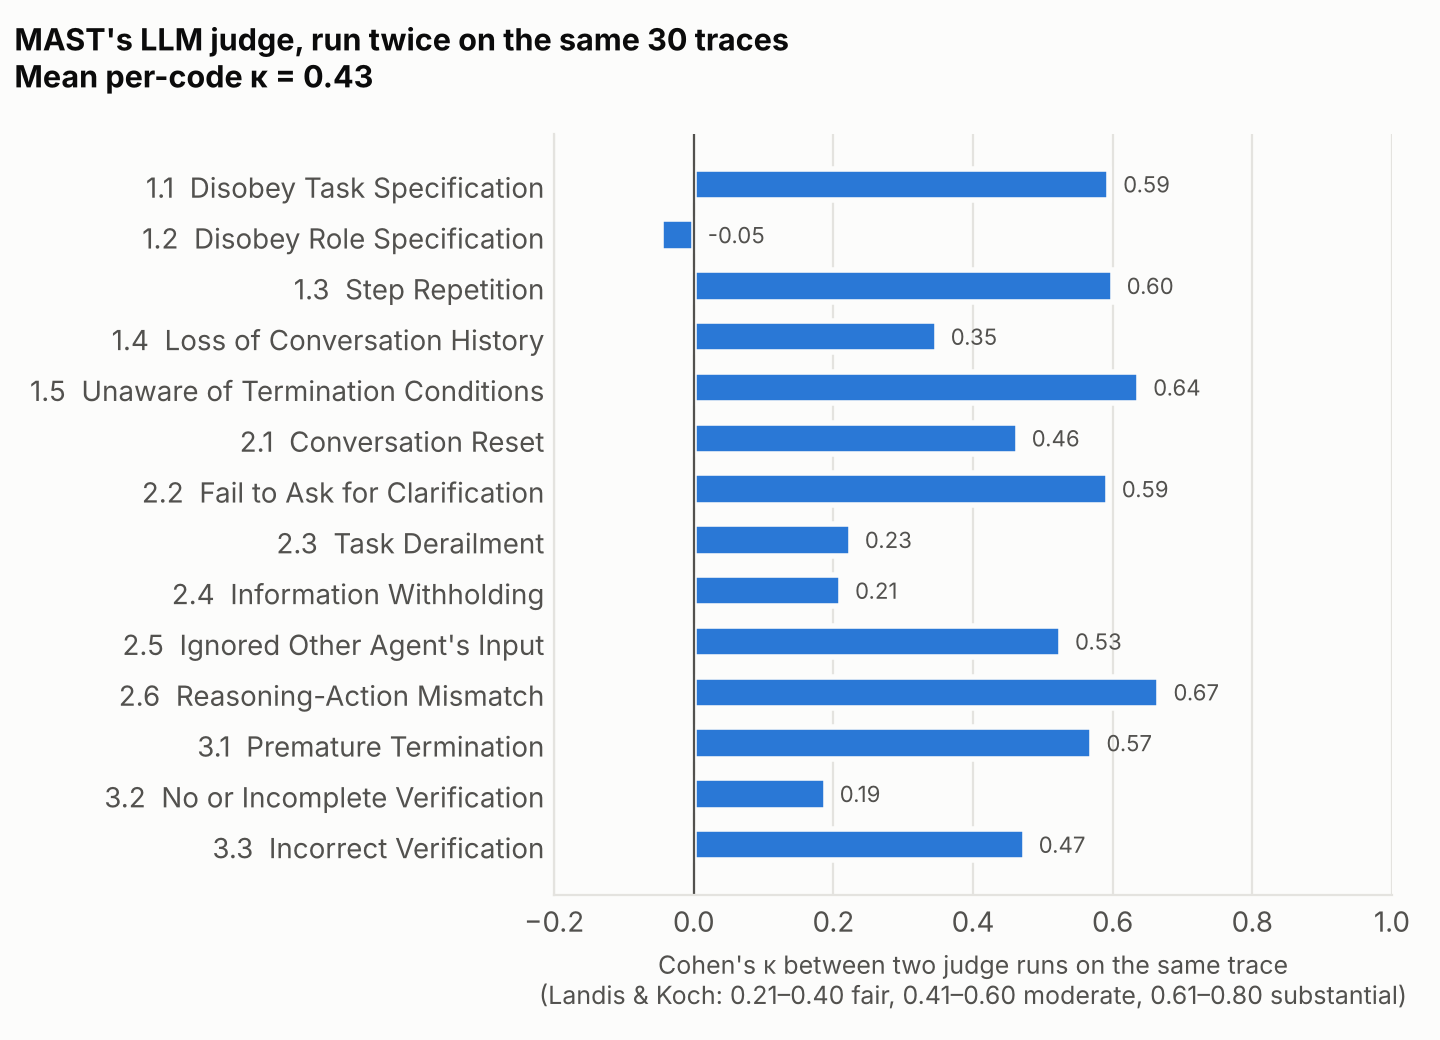
\includegraphics[width=0.6\linewidth]{mast_judge_test_retest.png}
\caption{Test--retest agreement of MAST's LLM judge on 30 byte-identical
Magentic-One traces labelled in two runs. Cohen's $\kappa$ per failure mode;
mean 0.43.}
\label{fig:retest}
\end{figure}

\paragraph{Metadata and logging.} The OpenManus traces are tagged as programming
tasks but are GAIA questions, and the AG2 ``GSM'' traces are GSM-Plus; both are
corrected. In 29 of 30 OpenManus logs the task is printed truncated (the agents
received the full text), and in one it was typed in and never logged; rendered
traces carry a note. Five runs have an empty task. MAST's human-labelled file holds
19 traces (not 21), and within every round different traces carry identical label
vectors, contradicting the original annotation sheets, so it is not used. Only 60
traces carry a benchmark verdict in the log (AppWorld and AG2 GSM-Plus).

\paragraph{Eligible pool.} The pool is 893 MAST-failed and 373 MAST-clean traces:
AG2 286 failed, MetaGPT 408, Magentic-One 127, AppWorld 27, OpenManus 27 and
HyperAgent 18 (Figure~\ref{fig:prevalence}). Four frameworks ran a single model,
and ``Claude'' carries no version number.

\begin{figure}[tbp]
\centering
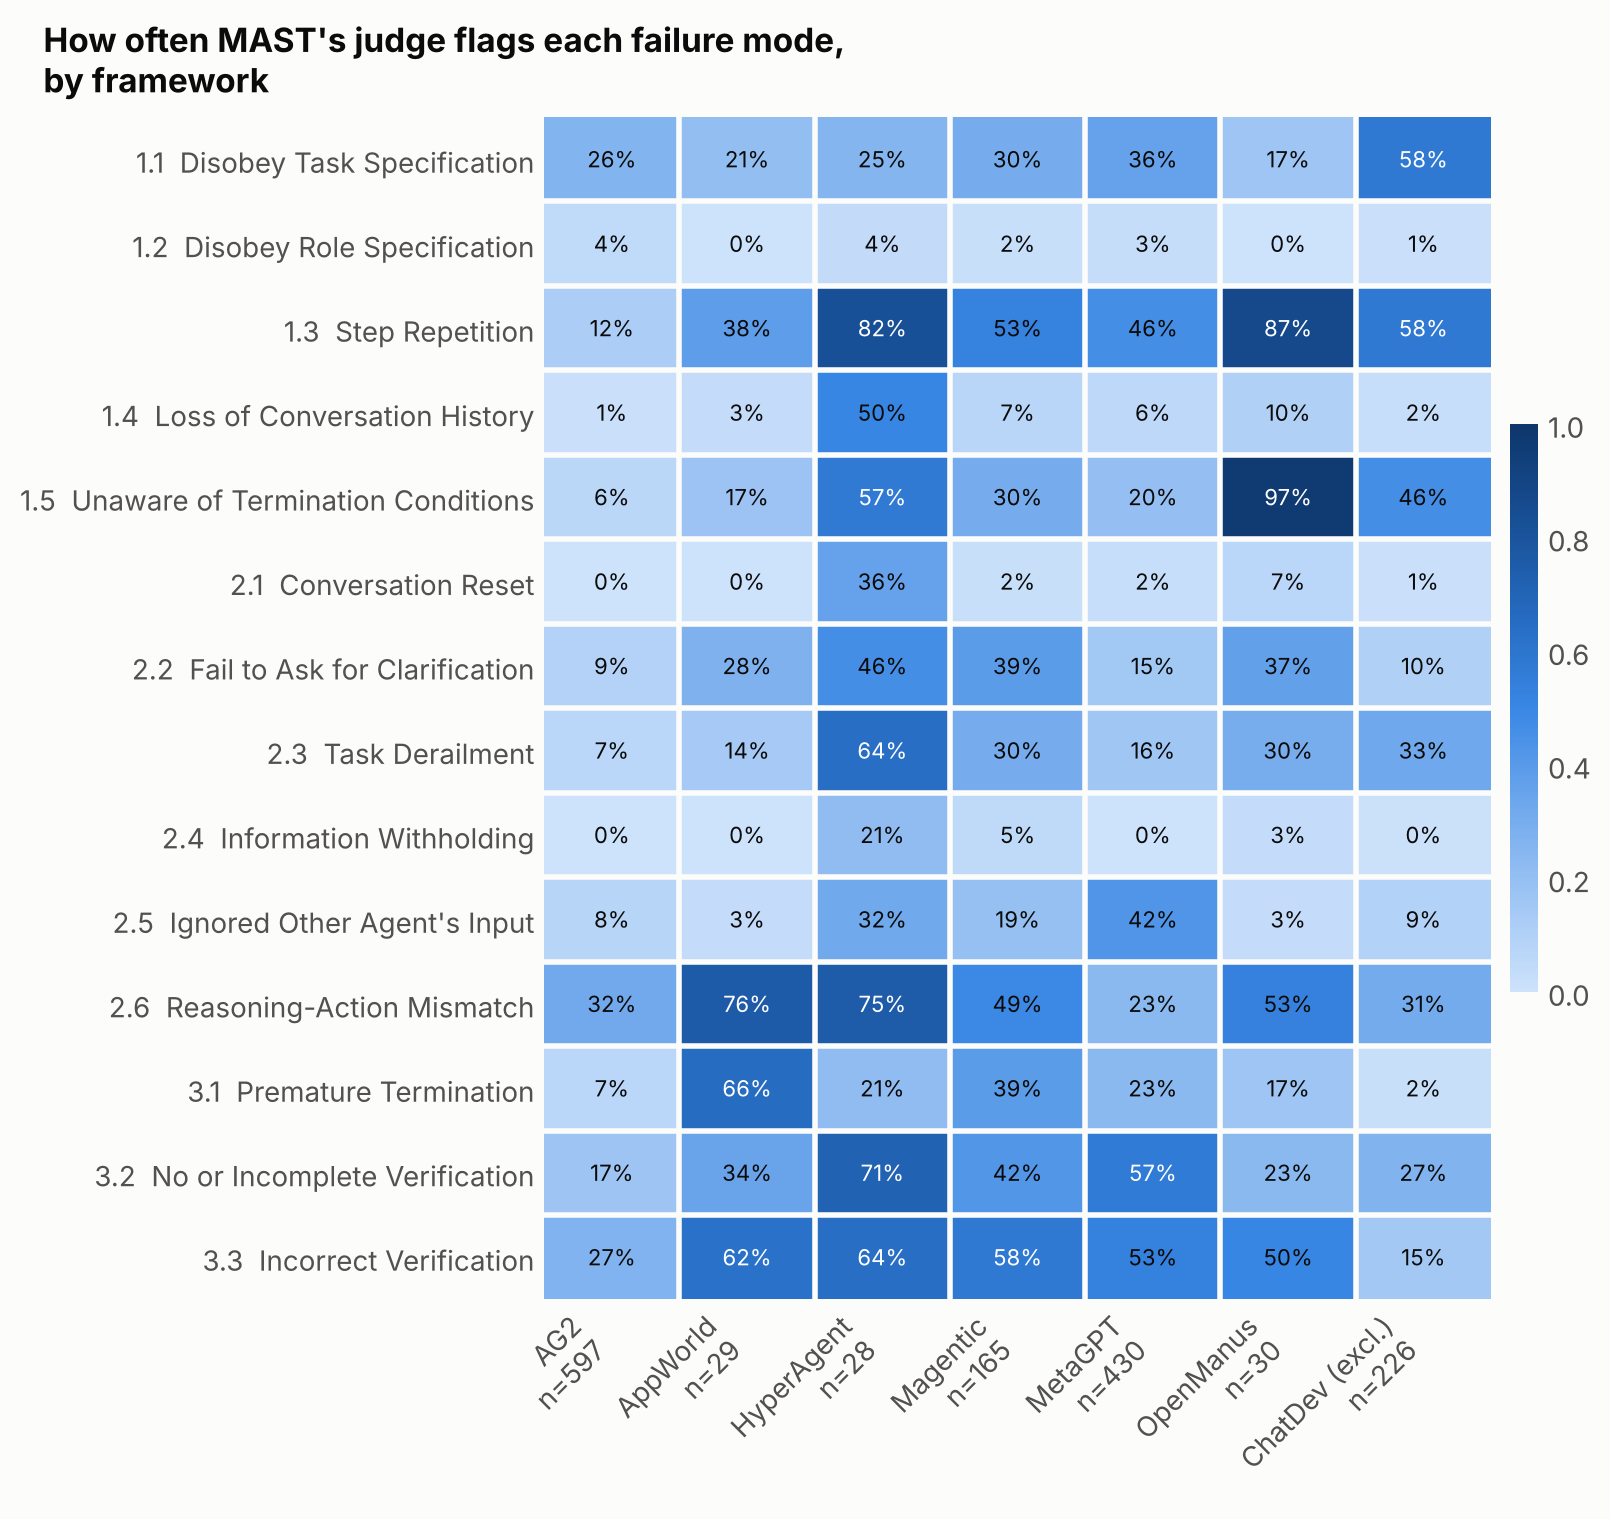
\includegraphics[width=0.58\linewidth]{mast_prevalence_by_framework.png}
\caption{Share of kept traces in which MAST's judge flags each failure mode, by
framework. ChatDev is shown for completeness but excluded from the study.}
\label{fig:prevalence}
\end{figure}

{\sloppy\paragraph{MAST's descriptions of the systems.} The documentation check found that
MAST describes MetaGPT as having an explicit verifier, whereas the logs show
MetaGPT's three-role example (425 of 430 traces follow its exact sequence), in
which a reviewer comments only on the tests and no agent revises the code. MAST's
HyperAgent traces come from a public SWE-bench submission dated September 2024 and
are labelled Claude-3.7-Sonnet, a model released later; the submission's metadata
names GPT-4o. The multi-agent AppWorld set-up and the AG2 MMLU team are MAST's own
constructions with unpublished prompts, and the Magentic-One version could be
inferred only from line numbers in a traceback.\par}

\section{Method Details}
\label{app:method}

\paragraph{Sampling and weights.} The bulk sample allocates traces across
frameworks and then across models within each framework by balanced allocation
(smallest groups first), excluding the frozen calibration set. Each trace is weighted by the number of eligible traces it
represents; shares use Wilson 95\% intervals on the Kish effective sample size
$n_{\mathrm{eff}}=(\sum w)^2/\sum w^2$.

\paragraph{Agreement.} Bootstrap intervals use 2{,}000 resamples of traces and are
omitted where either coder gave fewer than three positive or three negative
answers. The weighted deepest-layer $\kappa$ uses the full ordered label set, so
that distances are not distorted by absent levels.

\paragraph{Quote check.} Each quote is matched against its cited step after
normalising whitespace, quotation marks, capitals and markdown; an ellipsis splits a
quote into pieces that must appear in order. Quotes are classed as found in the
cited step, found in another step, not found, or citing a hidden or absent step.

\paragraph{Model-level comparisons.} L4.4 is not coded from traces. Instead,
patterns were compared across models with framework and benchmark held fixed
(MetaGPT on ProgramDev, Claude against GPT-4o; on ProgramDev-v2, Qwen against
CodeLlama; AG2 on GSM-Plus, Claude against GPT-4o). No MetaGPT group carried a
violation code. AG2's Olympiad traces, all from GPT-4o, carried one in 31\% of
failures, against none in its GSM-Plus and MMLU traces; there benchmark and model
are confounded. The groups are small and the comparisons exploratory.

\section{Further Tables}
\label{app:tables}

\begin{table}[tbp]
\centering
\caption{Evidence needed to code each AFACS layer, and the corresponding
information category in Ezell et al.~\cite{ezell2025incident}.}
\label{tab:evsource}
\small
\begin{tabular}{@{}L{3.4cm}L{6.2cm}L{4.6cm}@{}}
\toprule
Layer & Evidence needed & Ezell et al.\ category\\
\midrule
L1 unsafe acts, L2 preconditions & The trace: messages, actions, tool outputs & Activity logs; tool information\\
L3 supervision & The trace, the task specification and the system prompt & Activity logs (system and user prompts)\\
L4.1--L4.3 design, process & The trace and what is known of the system's design & System documentation; tool information\\
L4.5 operation set-up & The trace and what is known of how the run was launched and configured & Activity logs (user prompts); system configuration\\
L4.4 model development & Developer records: training and reward specifications, change logs, version or checkpoint comparisons & System documentation and change logs; system artefacts; model access\\
\bottomrule
\end{tabular}
\end{table}

\begin{table}[tbp]
\centering
\caption{Number of Ezell et al.'s eighteen information items each framework's
logs provide. Applicable excludes items that do not arise in these benchmark
runs (e.g.\ tool information for agents that use no tools).}
\label{tab:info}
\small
\begin{tabular}{@{}lrrrrr@{}}
\toprule
Framework & Traces & Applicable & Present & Partial & Absent\\
\midrule
AppWorld & 29 & 18 & 8 & 5 & 5\\
Magentic-One & 165 & 17 & 6 & 6 & 5\\
OpenManus & 30 & 17 & 6 & 4 & 7\\
HyperAgent & 28 & 17 & 5 & 5 & 7\\
AG2 & 597 & 15 & 2 & 5 & 8\\
ChatDev & 226 & 14 & 6 & 5 & 3\\
MetaGPT & 430 & 10 & 2 & 3 & 5\\
\bottomrule
\end{tabular}
\end{table}

\begin{table}[tbp]
\centering
\caption{Where the framework expects MAST's modes to fall in AFACS, stated before the pilot.}
\label{tab:expect}
\small
\begin{tabular}{@{}L{5.8cm}L{9.4cm}@{}}
\toprule
MAST mode & Expected AFACS location\\
\midrule
1.1 Disobey task specification & Spread: L3.4, L1.E2 or L1.E3, L1.V, or L4.5 (a run set up with no task)\\
1.2 Disobey role specification & L4.1 role design, or L1.E2 / L1.V\\
1.3 Step repetition & L1 act, with L3.3 where a supervisor could have broken the loop, and L4.1 (no termination logic)\\
1.4 Loss of conversation history & L2.2 agent state, with L4.2 context limits\\
1.5 Unaware of termination conditions & L4.1 termination logic, or L1.E2\\
2.1--2.5 Inter-agent misalignment & Mostly L2.3 coordination; 2.2 also L3.4\\
2.6 Reasoning--action mismatch & L1.E1 (sound intention, faulty execution), or L1.V\\
3.1 Premature termination & L1.E2, or L1.V (false claim of completion), with L3.1\\
3.2 No or incomplete verification & By whose job it was: L1 (incl.\ L1.V1 routine skipping), L3.1, or L4.1/L4.3\\
3.3 Incorrect verification & L3.1, L1.E2 or L1.E3\\
\bottomrule
\end{tabular}
\end{table}

\section{Further Worked Examples}
\label{app:cases}

\paragraph{A violation graded on the act (AG2).} In
\code{AG2\_Olympiad\_GPT4o\_\_150} the assistant is told to use Python for
calculations, wait for the results, and box its answer only after the queries have
run (S1). It reasons informally, then writes code headed ``Perform
calculation/verification'' in which the answer is assigned as a constant and
printed, and it boxes that number before the code has run (S2). The proxy returns
the constant (S3), and the assistant presents it as the outcome of its analysis
(S4). All three runs code \code{L1.V2} with the evidence graded \emph{inferred}:
nothing in the assistant's words acknowledges that the ``verification'' is empty,
but the act is hard to read as accidental. One run noted that a reviewer could
code it as a decision error only, which is the judgement the grade leaves visible.
Whether the answer is wrong cannot be told from the log.

\paragraph{A run with no task (MetaGPT).} In
\code{MetaGPT\_ProgramDev2\_GPT4o\_\_099} the task text is empty (S2). The coder
writes a placeholder (S3), the tester writes template tests for a function that
does not exist (S4), and the reviewer asks for more specific test inputs without
mentioning that there is no task (S5). MAST labels the trace FM-1.1 Disobey Task
Specification and FM-2.2 Fail to Ask for Clarification, but there was no
specification to disobey: condition (1) of the violation rule cannot hold. The
deepest factor is the run's set-up, L4.5 Operation set-up.

\end{document}
